\chapter{Generative Pattern Database}
% TODO: investigate the effect of clustering data into regions before applying gen model
Three main challenges in the context of data dissemination in CIDS were identified. First, intrusion related data is usually of sensitive nature. Thus, the exchange mechanism must not compromise any policies and regulations related to data \textit{privacy}. At the same time, the usability of the data has to be preserved. Second, the data that is subject of the exchange may exhibit large volumes. That constitutes a challenge, since the dissemination is desired to be executed with \textit{minimal overhead} in a timely and scalable fashion. Lastly, the \textit{interoperability} of the CIDS with existing local IDS is an important aspect that influences the practical adoption into security architectures.

In summary, existing approaches for data dissemination mainly provide mechanisms for exchanging alert data or single attributes, e.g. IP addresses, as they focus on the correlation of intrusion detection incidents that originate from different sensors. The exchange of actual training data is neglected, possibly due to high data volumes. Thus, these systems lack of mechanisms for the extraction and global persistence of novel attack patterns, e.g. from zero day exploits, that can be used for the training of an intrusion detection sensor.

The approach that is presented in this chapter exchanges attack patterns by sharing generative machine learning models that have been trained on partitions of similar data points. Such a model-based dissemination enables the receiving side to sample a synthetic dataset that enhances existing local datasets. This provides two main advantages. First, no original data leaves a local network and therefore does not violate any privacy restrictions. Second, the data is compressed considerably by representing it in form of a generative model. In order to make that mechanism scalable, the monitored data is clustered using random projections. This way, similar data points are partitioned into globally common clusters, which is exploited as a data parallelism mechanism. Given that, bursty workloads can be served effectively in a cloud deployment. Furthermore, this mechanism enables a similarity-based correlation of distributed intrusion events. The integration of both a similarity based correlation of intrusion incidents and a mechanism for sharing attack knowledge makes it possible to extract novel patterns of distributed attacks and provide them globally within the CIDS, resulting in an improved attack detection.

While Section \ref{sec:system_architecture} gives a high-level overview of the proposed architecture and its main processing primitives, details on the specific algorithms and strategies of the main services are described in Sections \ref{sec:local_indexing} to \ref{sec:classifier_fitting}.

\section{High Level Overview}\label{sec:high_level_overview}

Several members exist in the CIDS, each of which manages an isolated IDS. Every IDS operates according to a specific set of rules, that is essentially based on the content of a local database. The goal of the generative pattern database is to close the knowledge gaps of local databases and thus increase the detection rate of associated IDSs. By providing a \textit{global view} on all local databases, individual IDSs can benefit from the collective knowledge of the CIDS.

Section \ref{subsec:example_integration} starts with a reference example to illustrate the idea that is described above and discusses the integration of the CIDS into existing infrastructures. Subsequently, Section \ref{subsec:clustering} and Section \ref{subsec:filtering_and_compression} show the key concepts that enable data distribution and correlation under the given requirements. Finally, Section \ref{subsec:global_view} combines the individual elements to present the strategy for the creation and usage of the global view.


% The global view is a collection of transformed information from local intrusion detection datasets. 

% Before any data is transferred from a local network of a member of the CIDS to the global view, it is clustered, filtered and compressed (\textit{Privacy} and \textit{Minimal Overhead}). Upon each update on the global view, a synchronization from the global view to each local view of all members is initiated.  In this way, the accumulated global knowledge is shared with individual members enriching their local databases, which form the backbone of their attack detection.


% Section \ref{subsec:high_level_architecture} explains how this approach can be integrated into existing IDS architectures and introduces the key features and techniques that enable a data dissemination and correlation which meets the challenges described in section \ref{subsec:challenges}. Subsequently, details on the rules and processes for creating the global view are presented in section \ref{subsec:global_view}.

\begin{figure}[t!]
    \centering
    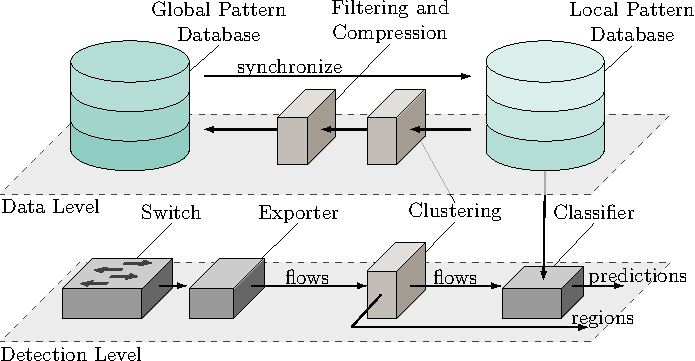
\includegraphics[width=0.8\linewidth]{tikz/high_level_architecture.pdf}
    \caption{Integration of the approach into a generic NIDS.}
    \label{fig:high_level_architecture}
\end{figure}



\subsection{Example Integration}\label{subsec:example_integration}
An exemplary integration of the CIDS into a generic NIDS is shown in Figure \ref{fig:high_level_architecture}. The shown NIDS consists of three components, which can be found on the detection layer. A flow exporter computes statistical flow features based on the network packets of a switch. A discriminative model serves as a classifier that operates on the specific feature set that the exporter extracts. After completing the training of a classifier instance on a given dataset, it is deployed within the detection pipeline. There, the classifier receives a stream of network flows and predicts them.

The CIDS mainly integrates at the data level, where the training data for the classifier is provided by the \textit{local pattern database}. At this point, the local pattern database only contains the \textit{local view} of the intrusion detection data from that particular member. In order to provide a global view for that member, a synchronization process between its local pattern database and the \textit{global pattern database} has to be initiated. Before the data is transferred to the global pattern database, is subject to a set of clustering, filtering and compression operations. This way, data privacy is maintained and the overhead is minimized by reducing the data volume. On the receiving side, the global pattern database combines data from all members to a global view.

Upon each update of the global pattern database, the new state of the global view is synchronized to each local pattern database and subsequently enhances the classifier on the detection level by extending the local intrusion detection dataset. Furthermore, an identical clustering operation as on the data level is applied on the detection level. Each incoming flow is assigned to a certain cluster, which is referred to as \textit{region}. While the predictions from the classifier are suitable for detecting attacks that are known to the CIDS, regions are leveraged for the detection of novel data patterns and similarity-based correlations that uncover stealthy attacks, which are executed on the resources of multiple CIDS members simultanously.

\subsection{Clustering}\label{subsec:clustering}

Since the results of the clustering operation should be consistent, while its execution is distributed among all members of the CIDS, an unsupervised algorithm with few parameters for initialization has to be selected. Additionally, the algorithm should be scalable, since it is to be applied on whole databases on the data level and on streams of live data on the detection level. Given these requirements, random projection is a good choice. 


By using random projection, real data points are clustered according to their angular distance. Furthermore, the projection result is a binary string, which can be used for storing similar data points into a common bucket of a hash table by using the binary string as an index. In the context of the generative pattern database, the combination of random projections and hash tables is exploited as the main controlling primitive for data persistence and retrieval. Instead of using randomly selected projection planes, a shared seed results in the application of a common projection function among all members of the collaboration. In other words, similar data points from different datasets are indexed to a common global bucket, i.e. region. Each region is subject to the transformations individually, which is utilized as a data parallelism mechanism. Thus, this approach is natively suited for cloud deployments where bursty workloads can be served effectively. Lastly, this mechanism enables a similarity-based correlation of distributed intrusion events. As incoming data is monitored on the detection level, the clustering is applied, which results in a pattern that can be used for novelty checks or global occurrences within the CIDS.

\subsection{Filtering and Compression}\label{subsec:filtering_and_compression}

Two types of data are extracted within individual regions. First, metadata of local datasets is collected by counting label occurrences, which serve as indicator for determining if the respective region needs to be subject to the second extraction type. Second, models that are trained with generative algorithms on local attack data are the exchange medium for disseminating information within the CIDS. This provides two main advantages. For one, no original data leaves a local network and therefore does not violate any privacy restrictions. For another, the data is compressed considerably by representing it in form of a generative model. 

\subsection{Global View}\label{subsec:global_view}

\begin{figure}[b!]
    \centering
    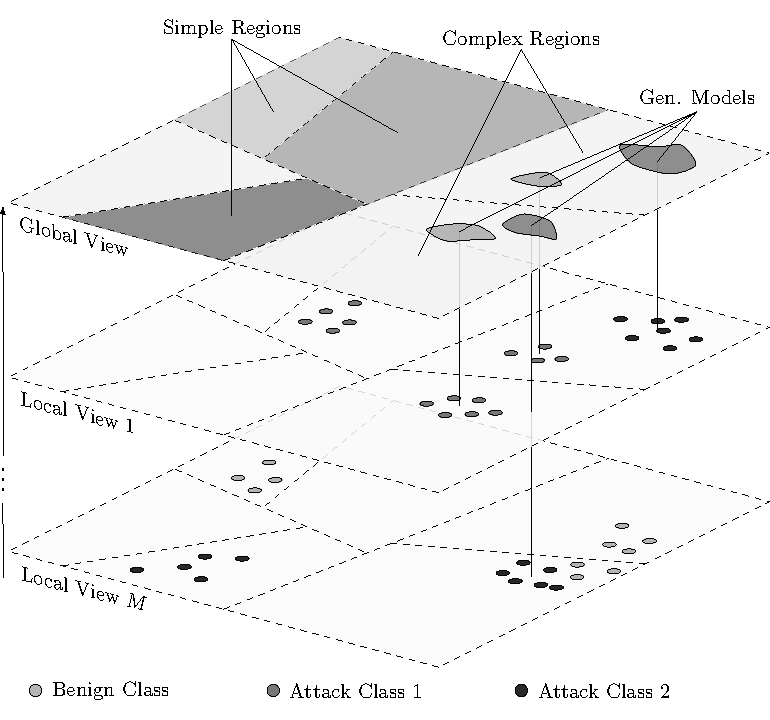
\includegraphics[width=0.8\linewidth]{tikz/global_view.pdf}
    \caption{Building the global view by combining $M$ local views.}
    \label{fig:global_view}
\end{figure}


As shown in Figure \ref{fig:global_view}, each view is partitioned by a common projection function into an identical set of regions. Each local view contains original datapoints from its respective dataset. In this example, there exist three different classes globally, which occur differently in each local dataset. Examining a specific region, the combination of unique classes within all local views determines its complexity on a global level. If a region contains more than one class, it potentially exhibits a non-linear decision boundary, hence it is called complex. Otherwise, a region is called simple. Attack data within a complex region, seperated by its label, is used as training data for a generative algorithm. Subsequently, the resulting model is transferred to the global view. 


A synchronization process disseminates the region complexity estimations and the generative models to all local views. By sampling data from multiple generative models, a synthetic dataset is assembled, which is blended into the respective local datasets for enhancing the subsequent training of a discriminative model.

\section{System Architecture} \label{sec:system_architecture}

% Provide a general view on main components and their tasks and interfaces; how is this system supposed to work; how do the components interact with each other
% Specify important definitions on components and data formally


\begin{figure}[b!]
    \centering
    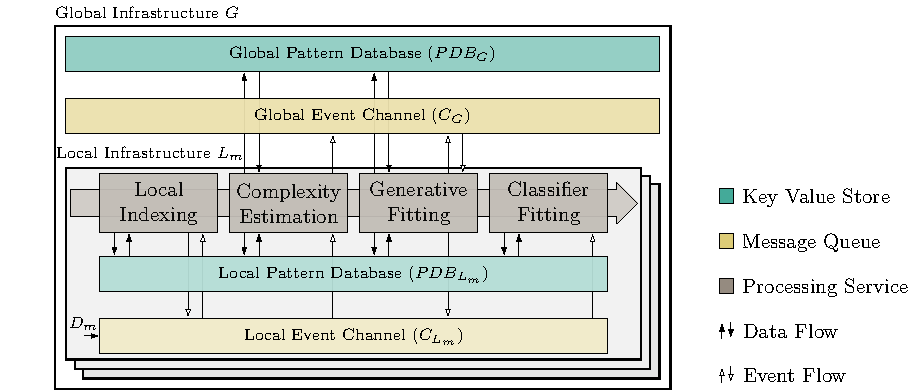
\includegraphics[width=1\linewidth]{tikz/detailed_architecture.pdf}
    \caption{High level CIDS architecture.}
    \label{fig:detailed_architecture}
    \end{figure}

    
    Logically, the proposed CIDS exhibits a hierarchical architecture (see Figure \ref{fig:high_level_architecture}). For one, the global infrastructure $G$ represents the collection of $M \in \mathbb{N}$ CIDS participants and their knowledge on an abstract level. For another, it provides specific services, that are globally available to each local infrastructure $L_m, m \in \{1, \dots, M\}$ that includes all CIDS components and processes within the IT infrastructure boundaries of a corresponding CIDS member. Each local infrastructure $L_m$ agrees to a specified feature extraction process that provides the monitoring data $\bm{X} \subset \mathbb{R}^d$ for the attack detection. Single data points of the monitoring data are referred to as $\bm{x} \in \bm{X}$ with a total number of features $d = |\bm{x}| \in \mathbb{N}$. In addition, the set of targets $Y \subset \mathbb{N}$ with instances $y \in Y$ is known and registered by every local infrastructure $L_m$. Furthermore, every $L_m$ provides an individual training dataset $D_m= \{(\bm{x}_n, y_n): 1 \leq n \leq N_m\}$ of size $N_m = |D_m| \in \mathbb{N}$. CIDS communication across local boundaries occurs exclusively in a vertical direction. Thus, the exchange of information between individual $L_m$ takes place indirectly via the global pattern database $(PDB_G)$ and the global event channel $(C_G)$. Each $L_m$ includes a local pattern database $(PDB_{L_m})$, a local event channel $(C_{L_m})$ and an event-based data processing pipeline that consists of four services.

    \begin{table}[b]
        \centering
        
\begin{tabular}{ll} 
    \toprule
    \textbf{Notation} & \textbf{Description}             \\ 
    \midrule
    $G$                     & Global Infrastructure            \\
    $L_m$                   & Local Infrastructure $m$             \\
    \midrule
    $PDB_G, PDB_{L_m}$                   & Global Pattern Database, Local Pattern Database of $L_m$             \\
    $C_G, C_{L_m}$                     & Global Event Channel, Local Event Channel of $L_m$                    \\
    \midrule
    $M \in \mathbb{N}$      & Total number of CIDS participants         \\
    $m \in \{1, \dots, M\}  $         & Local Infrastructure Identifier  \\
    \bottomrule
\end{tabular}

        \caption{Summary of the architecture notation.}
    \end{table}

\subsection{Pattern Database} \label{subsec:pattern_database}

% what are the tasks of a pdb
depending on the scope (either local or global), different tasks are considered
local pdbs store intrusion detection datasets and corresponding metadata of the respective member; 
global pdbs store global metadata (combined information of local datasets) and the generative models


Each instance of a pattern database $(PDB)$ is realized as a key-value store. For the following algorithm descriptions, a $PDB$ is treated as a hash table as defined in Section \ref{subsec:hash_table}, that is referred to by replacing its function variable with the identifier of the corresponding database, e.g. $PDB_G(k)$ being a specific slot or hash value related to a key $k$ in the global pattern database. Note that if a specific hash function is already used to construct a key (e.g. Random Projection), the hash table will internally apply a distinct hash function on the key to ensure even distribution across the slots.

\subsection{Event Channel} \label{subsec:event_channel}
Event channels provide a topic-based publish-subscribe messaging mechanism that is mainly used to distribute workloads among the service instances in the processing pipeline. Via the messaging system, service instances receive and emit events, on which upon the respective operations are triggered. Changes in a pattern database result in responses that in turn are leveraged as the respective events. In this fashion, updates are propagated throughout the processing pipeline, ensuring a timely consistency among the pattern databases.

\subsection{Processing Pipeline} \label{subsec:processing_pipeline} 
Local and global pattern databases serve exclusively as data sources and sinks for operations. The only exception is the initial import of datasets $D_m$ into the \textit{Local Indexing} service via the messaging system.




\newpage
\section{Local Indexing} \label{sec:local_indexing}

\begin{figure}[b]
    \centering
    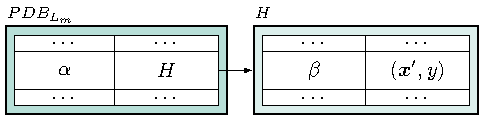
\includegraphics[width=1\linewidth]{tikz/indexing.pdf}
    \caption{Nested indexing in a local pattern database.}
    \label{fig:indexing}
\end{figure}

The local indexing service listens on $C_{L_m}$ for new data points from $D_m$. First, data points are buffered until a defined batch size is released. Subsequently, the batch $X$ is scaled to the range $[-1, 1]$ by applying a feature-wise min-max normalization, given by

\begin{align*}
    \bm{X}' = \frac{\bm{X}-min(\bm{X})}{max(\bm{X}) - min(\bm{X})} \cdot (b - a) + a, \quad
    \setlength\arraycolsep{2pt}
    \begin{array}{lr}
        a = &-1 \\
        b = & 1    
    \end{array}.
\end{align*}

After that, each element $\bm{x}' \in \bm{X}'$ is subject to both a \textit{GRP} $h$ with a global seed for the initialization of the projection plane $\bm{M}$ (see Section \ref{subsec:gaussian_random_projection}) and a non-cryptographic hashing function $g$ (see Section \ref{subsubsec:non-cryptographic-hashes}). The \textit{GRP} clusters the data by mapping similar data points $\bm{x}'$ to the same hash value. The non-cryptographic hashing function on the other hand serves as a mechanism for deduplicating identical $\bm{x}'$. In order to insert a pair $(\bm{x}'_n, y_n) \in D_m$ into the $PDB_{L_m}$, at first two keys $k_\alpha, k_\beta \in K$ are constructed as

\begin{align*}
    k_\alpha(\bm{x}'_n, y_n) &= p_x \doubleplus h(\bm{x}'_n) \doubleplus y_n,\\
    k_\beta(\bm{x}'_n) &= g(\bm{x}'_n),
\end{align*}

where $\doubleplus$ indicates the concatenation operator and $p_x$ describes an arbitrary prefix constant. Secondly, if not already present, a hash table $T_{m_n}$ is created and inserted into the slot $PDB_{L_m}(k_\alpha(\bm{x}'_n, y_n))$. Finally, $(\bm{x}'_n, y_n)$ is hashed into the slot $T_{m_n}(k_\beta(\bm{x}'_n))$. That nested indexing is depicted in Figure \ref{fig:indexing}. Since a particular $h(\bm{x}')$ is a cluster of similar data points, we refer to it as a \textit{region}. Therefore, every region is represented by one or more hash tables $T_{m_n}$, each of them containing data points that belong to the same label. Each execution of that insert operation is executed idempotently, such that the pattern database only returns a response upon the insertion of new data points. For each response, the corresponding region $h(\bm{x}'_n)$ is sent into the local event channel $C_{L_m}$ as an event that indicates a change on a certain cluster within the local pattern database.
\newpage
\section{Complexity Estimation} \label{sec:complexity_estimation}

A region is said to be complex, if it contains more than one unique label. Otherwise, a region is simple. Since the data within a region already represents a cluster, the existence of multiple classes indicates a more complex decision boundary. On that basis we differentiate how a region is processed in the subsequent services of the pipeline. Furthermore, the complexity state of a region may vary, depending on the scope it is observed. Note that since the projection matrix $\bm{M}$ is initialized with the same values in every $L_m$, all hashes that were computed by $h$ are globally comparable. This means that similar data points from different datasets, e.g. $\bm{x}_i \in D_1$ and $\bm{x}_j^* \in D_2$ may be hashed to the same region $h(\bm{x}_i) = h(\bm{x}^*_j)$. However, it is also possible that that the corresponding labels $y_i \in D_1$ and $y^*_j \in D_2$ are not equal and therefore lead to a different global view on that region's complexity state. Given that, the complexity estimation module acts as a bridge between the local and global components and answers the question, which regions are considered to be complex in a global context. First, an event containing a region $h(\bm{x}'_n)$ is received. This event is then used for retrieving the set of unique labels $Y_{h(\bm{x}'_n)}$ for that particular region stored at $PDB_{L_m}$, which is defined as

 \begin{align*}
    \bigcup_{y \in Y} \! \Bigl\{ y_n \! \in \! \bigl\{T_{m_n}\bigl(k_\beta(\bm{x}'_n)\bigl)\bigl\} : \! T_{m_n} \! \! \in \! \bigl\{PDB_{L_m}\bigl(k_\alpha(\bm{x}'_n, y) \bigl)\bigl\}\Bigl\}.
 \end{align*}

 Next, a key $k_\gamma \in K$ is constructed by concatenating an arbitrary prefix constant $p_y$ with the region $h(\bm{x}'_n)$ and the id of the current local infrastructure $m$:

\begin{align*}
    k_\gamma(h(\bm{x}'_n), m) = p_y \doubleplus h(\bm{x}'_n) \doubleplus m.
\end{align*}

 Then, $Y_{h(\bm{x}'_n)}$ is inserted into the global pattern database at the slot $PDB_G(k_\gamma(h(\bm{x}'_n), m))$. The global complexity $c_{h(\bm{x}'_n)} \in \{0, 1\}$ is determined by combining the respective label sets from all local infrastructures and evaluating its cardinality:
 
 \begin{align*}
    c_{h(\bm{x}'_n)} = \Bigl| \bigcup_{m \in M} \Bigl\{ PDB_G\bigl(k_\gamma(h(\bm{x}'_n), m)\bigl) \Bigl\}\Bigl| > 1.
 \end{align*}

 Finally, the state $c_{h(\bm{x}'_n)}$ is inserted in the global pattern database by constructing a key $k_\kappa \in K$ with a prefix constant $p_c$ and the region $h(\bm{x}'_n)$ as

 \begin{align*}
     k_\kappa(h(\bm{x}'_n)) = p_c \doubleplus h(\bm{x}'_n)
 \end{align*}

and storing it in the slot $PDB_G(k_\kappa(h(\bm{x}'_n)))$. If the state has changed, a response is returned and the corresponding region $h(\bm{x}'_n)$ is sent as an event into the global event channel $C_G$.

\newpage
\section{Generative Fitting} \label{sec:generative_fitting}

\begin{algorithm}
    \caption{Main Loop}
    \label{alg:generative_fitting}
    \algsetup{indent=2em}
 
    \begin{algorithmic}[1]
        \REQUIRE Regions $R_{\text{in}}$
        \ENSURE Regions $R_{\text{out}}$

        \STATE $m \leftarrow$ getID()
        \FORALL{$r$ in $R_{\text{in}}$}
            \STATE $k_\kappa \leftarrow \text{concatenate}(p_c, r)$
            \STATE $c_r \leftarrow PDB_G[k_\kappa]$ % get complexity estimate for that region
            \STATE $k_\delta \leftarrow \text{concatenate}(p_y, r, m)$
            \STATE $Y_r \leftarrow PDB_G[k_\delta]$ % get label set of region from global PDB
            
            \FORALL{$y$ in $Y_r$}
                \STATE $k_\omega \leftarrow \text{concatenate}(p_d, r, y, m)$ 
                \IF{$c_r = 0$}
                    \STATE delete model in $PDB_G[k_\omega]$
                \ELSE
                    \STATE . % retrieve flows
                    \STATE . % fit gen model
                \ENDIF
            
            \ENDFOR          
 
            
        \ENDFOR

    \end{algorithmic}
 \end{algorithm}

% ALGO 3: Generative Fitting
% get regions from communication channel

% for each region in R
%   - get complexity estimate for that region
%   - if region is simple and model is available in that region:
%       evict model from database
%   - else (model is complex)
%       retrieve flows from every HashTable that belongs to that region
%   - fit generative model() // ALGO 3.1
%   - persist model(dataset)


% ALGO 3.1: Dataset preprocessing
% catalogs = {}
% for label in dataset:
%   if label is not benign:
%           // split into binary (filter the label that is to be learned into on chunk and the rest into another chunk)
%           // upsample
%           // model_selection()

% ALGO 3.2: Model Fitting and Selection
% n_components <- collection of params[1 - X.shape//2, 2er schritte]
% cov_types <- collection of params[spherical, diag, full]
% for each component in n_components:
%   for each cov_type in cov_types:
%       X_pca <- pca.fit_transform(X)
%       gmm.fit(X_pca)
%       bic <- gmm.bic(X_pca)
%       // evaluation step
%           - synth. samples from gmm (how many?)
%           - inverse transform pca on these samples
%           - create training dataset
%           - create testing dataset
%           - train DecisionTreeClassifier with train dataset
%           - test DTClf with test dataset
%           - write balanced accuracy score into catalog
%           - write bic into catalog
% sort list_of_gmms by bic (lowest is best)
% sort list_of_gmms by acc (highest is best)
% return best gmm

\newpage
\section{Classifier Fitting} \label{sec:classifier_fitting}

The objective of the classifier fitting service is to provide the local IDS with the latest classification model trained on both original local data and synthetic global data. After each change to the generative models in the global pattern database made by the previous service, an event is sent into the communication channel. Within a defined time window, all such events are collected. If at least a single event was collected, the classifier fitting service is initiated and begins with assembling a training dataset. For this task, all original data are first loaded from the local PDB. Then, all generative models are loaded sequentially from the PDB and provided. n the process, synthetic data is generated in the amount that was also originally found in the corresponding region. After each sampling, the synthetic data is transferred from the lower-dimensional subspace to the original data space by the inverse function of the original PCA operation. Subsequently, the normalization operation is also reversed for both the original and the synthetic data by loading the corresponding parameters that were used to normalize a batch from the PDB. 

\begin{algorithm}
    \caption{Dataset Assembly and Classifier Fitting}
    \label{alg:classifier_fitting}
    \algsetup{indent=2em}
 
    \begin{algorithmic}[1]
        \REQUIRE Region Update Event $r$
        \ENSURE Model Update Notification

        


    \end{algorithmic}
 \end{algorithm}



% load the local dataset

% iterate through all regions and retrieve the respective model parameters

%       rebuild GMM and PCA models by deserialization and putting in parameters
%       sample as many samples per (GMM,PCA) as originally indexed into the respective region-label-infrastructure combination
%       collect (sample,label)-pairs in a collection

% combine local dataset and synthetic dataset
% shuffle, split
% fit Ensemble of DecisionTrees (RandomForest) on combined dataset
% serialize DecisionTree model and put into PDB
% put an event into local communication channel
% local IDS receives Event and retrieves lates DT-Model and puts it into the decision pipeline

